%!TEX root = thesis.tex

\chapter{Introduction}

% \section{Brief History of Social Choice Theory}

	Election systems resembling what we know today date back to around 508 BC in Athens, Greece. The greeks used both the majority rule and the plurality systems which are very simple systems with one disadvantage being that each voter can only voice a preference for a single candidate. A more accurate way to represent each voter's opinion is with a ranked list of all candidates so, for instance, if candidates tie for first place, the tie can easily be broken by looking at voters' second choice, and then the third choice can be taken into account, etc. We call this ranked list a preference list.

	There weren't many improved ideas for election systems until much later, in the 13th century when Ramon Llull studied election systems \cite{hägele2001llull}. In 1770 Jean-Charles de Borda independently proposed an election system similar to Llull's, now called the Borda count, as a way of electing members of the French Academy of Sciences \cite{borda1781mémoire}. In the Borda count system, each candidate receives points based on their rank in each voter's preference list, with the winner being the candidate to receive the most points. Majority rule, plurality, and the Borda count are a some examples of voting rules, but there are many others, each with various strengths and weaknesses. Therefore, it is useful to compare them to each other. The most obvious criteria for a good election system is fairness \cite{chevaleyre2006issues}, because we would like the winning candidate to be the one which best represents the constituents' preferences. Fairness of an election system is easy to recognize if there are only two candidates: the candidate who is preferred by the majority of voters should win. But with a larger number of candidates, determining the fairness of an election system is not so obvious.

	Marquis de Condorcet, a contemporary of Borda, was interested in the fairness of voting systems and he proposed that the winning candidate be the candidate who would win a head-to-head election against each of the other candidates. Such a winner is known as the \emph{Condorcet winner}. Unfortunately, Condorcet also proved that a Condorcet winner does not always exist. Nevertheless, the Condorcet criterion was one of the first formal fairness criteria, and is still widely used today.

	In 1950, Kenneth Arrow, an American economist who was interested in the fairness of social welfare functions, made a large contribution to the field of Social Choice Theory with his impossibility theorem. Arrow's theorem \cite{arrow1950difficulty} (which he strengthened in 1963 \cite{arrow1963social}) demonstrates that no social welfare function can ``fairly'' convert the preferences of voters into a society-wide preference list. While ``fair'' is clearly subjective, he gave a list of basic properties which seem intuitively required for fairness:
	\begin{description}
		\item[Unrestricted domain (universality)] All individual preferences are allowed, and yield a valid group preference.
		\item[Independence of irrelevant alternatives] If all voters' preferences between alternatives $x$ and $y$ remain the same, the group preference between $x$ and $y$ is unchanged even if voters change their preferences regarding other alternatives.
		\item[Pareto principle (unanimity)] Unanimity of individual preferences implies a group preference. E.g. if all individuals prefer alternative $x$ to $y$, then the group will prefer $x$ to $y$.
		\item[Non-dictatorship] There is no voter whose preference always dictates the group preference.
	\end{description}
	Arrow proved that these properties are inconsistent: no voting system can satisfy all of these properties, hence, no social welfare function can be completely fair.

	The work done by Condorcet and Arrow is widely regarded as being foundational to the modern field of Social Choice Theory, and marks a transition from viewing social choice as a purely practical problem to a more rigorous theoretical study.


\section{History of Manipulation}

	One problem relating to the issue of fairness in social choice is that of manipulation (or strategic voting or tactical voting). Manipulation is when an individual purposefully misrepresents his preferences hoping to get a more favorable outcome in the election. For example, if a voter knows that his most preferred alternative has no chance of winning the election, he may instead say that he prefers a different alternative, so that even though his favorite alternative cannot win, at least his second choice alternative has a better chance of winning. This manipulation will benefit the voter but will not benefit society in general, because by lying about his preferences the voter has skewed the results of the election in his favor. Therefore, it is beneficial to search for ways to avoid manipulation in social choice.

	One way to avoid manipulation would be to devise a voting rule that is non-manipulable. Unfortunately, in 1973 the Gibbard-Satterthwaite theorem was published which states that every voting rule satisfying the following properties is subject to manipulation.
	\begin{description}
		\item[Non-dictatorship] (Defined above, in Arrow's theorem)
		\item[Non-imposition] Every alternative has the possibility of winning.
	\end{description}
	It would certainly seem that any reasonable voting rule would need to satisfy both of these criteria, hence, any reasonable voting rule is manipulable \cite{gibbard1973manipulation, satterthwaite1975strategy, duggan2000strategic}. This means that we cannot make manipulation impossible via a cleverly devised voting rule --- a rather disappointing prospect.

	% Begin rough draft

	Until this point in the history, social choice theory had been separate from computer science --- and indeed computer science was a very young discipline at this point. A new sub-field of social choice theory was spawned, computational social choice theory, which applies the studies of computer science to social choice theory. In 1989, Bartholdi, Tovey, and Trick proposed a computational barrier to manipulation in election systems \cite{bartholdi1989computational}. Instead of trying to make manipulation impossible, they endeavored to make it computationally intractable \cite{chevaleyre2007short}; even if a profitable manipulation exists it is of no use in practice if it is computationally infeasible to find. They were able to demonstrate that while many voting rules are easy to manipulate (a manipulation can be found in polynomial time), the problem of finding a manipulation for certain scoring rules is NP-complete. They called rules that can be manipulated in polynomial time \emph{vulnerable}, and those for which manipulation is NP-hard \emph{resistant}. For a formal definition of manipulation, see Definition.

	This ushered in a new way to approach social choice: from a computational footing. Bartholdi, Tovey, and Trick also studied the computational difficulty of finding a winner for various voting rules. For example, they showed that the Dodgson method mentioned above \cite{dodgson1876method} is actually infeasible to manipulate for the simple reason that figuring out the winner of the election is NP-hard. Therefore, it is not sufficient for a desirable voting rule to be hard to manipulate; it must also be also be efficient to determine a winner.

	In 1991, Bartholdi and Orlin \cite{bartholdi1991single} added to the above results by showing that the Single Transferable Vote (STV) rule was both resistant to manipulation, and quick to determine a winner. Although STV has problems of its own \cite{brams1982ams, doron1977single, fishburn1983paradoxes, holzman1989vote, moulin1988condorcet}, it is encouraging to see that it is possible for an efficient voting rule to resist manipulation.

	In 2002, Conitzer and Sandholm took a slightly different approach \cite{conitzer2002vote} (which they later extended \cite{conitzer2007elections}), studying coalition manipulation. Instead of a single voter manipulating an election, a group (coalition) of voters work together to manipulate an election. This vein of research has since been extended in various directions \cite{conitzer2003universal, elkind2005hybrid, faliszewski2006complexity, hemaspaandra2007anyone, procaccia2007multi, elkind2005small}.

	The work mentioned so far which attempts to erect a computational barrier to manipulation is encouraging, and may indeed provide ways to prevent manipulation in election systems. However it deals with the worst-case complexity of manipulation. In 2006, work by Conitzer and Sandholm \cite{conitzer2006nonexistence} along with that of Procaccia and Rosenschein \cite{procaccia2006junta} showed that while manipulation can be hard in the worst case, it is much easier in the average case. In the next few years more work was done to make this concern even more well-founded \cite{procaccia2007average, erdelyi2007approximating}. Work along these lines by Friedgut, Kalai, and Nisan \cite{friedgut2008elections} in 2008 is the main inspiration for this thesis, and has also spawned other work which will be discussed further in the Related Work chapter.















	We will now take an in-depth look at some of the results leading up to and related to our own. Unless the reader is familiar with this topic area, he should refer to the Preliminaries chapter for definitions of any of our notation, or to the cited paper for notation specific to that paper. In general, an election will consist of a SCF $f$, a set of $m$ alternatives $C$, $n$ voters, and a profile $P \subseteq L(C)^n$.

	Complexity theorists have analyzed many voting systems using computational complexity as a means of inhibiting manipulation \cite{bartholdi1989computational, hemaspaandra2009hybrid}. Friedgut, Kalai, and Nisan, on the other hand, took a probabilistic approach to this problem \cite{friedgut2008elections}. Instead of studying worst-case manipulation, they performed a probabilistic analysis of random manipulation. That is, instead of a voter intelligently manipulating an election, which can be difficult in terms of worst-case complexity, he simply chooses his manipulation randomly (if his most preferred candidate is not winning already). They proved that even a random manipulation will succeed with non-negligible probability. This is significant because no matter how hard it is in the worst-case to find a profitable manipulation, if it is trivial to find a random manipulation, that could be enough.

	More formally they defined a metric, \emph{manipulation power} $M_i(f)$, of voter $i$ on a social choice function $f$ to be the probability that $p_i'$ is a profitable manipulation by voter $i$, where $p$ is a profile and $p_i'$ is a preference list which are both chosen uniformly at random. Their main result is that there exists a constant $C$ such that for 3 alternatives, $n$ voters, and a neutral social choice function $f$ which is $\epsilon$-far from dictatorship ($\epsilon > 0$) then

	\begin{align*}
		\sum_{i=1}^n M_i(f) \ge C \epsilon^2
	\end{align*}

	This means that when $\epsilon$ is fixed --- it is once a voting rule is determined --- then some voter has more than his share (a non-negligible amount) of manipulation power: $\max_i M_i(f) \ge \Omega(\frac{1}{n})$ \cite{friedgut2008elections}.

	Besides the unfortunate limitation of 3 alternatives, these results are incredibly general. The only assumptions are the \emph{impartial culture} assumption, that votes are selected uniformly at random, and the neutrality of the social choice function. The neutrality assumption was removed by Friedgut, Kalai, and Nisan in 2011 \cite{friedgut2011quantitative}.

	However, these results apply only to elections with a maximum of 3 alternatives, which is not useful for most practical applications, and is less satisfactory than a general solution from a practical and theoretical standpoint. Therefore many people have worked to generalize these results.

	In 2008 Xia and Conitzer were able to prove a similar theorem for any number of candidates, but instead of neutrality they assumed 5 other conditions for the voting rule \cite{xia2008sufficient}:

	\begin{description}
		\item[Homogeneity] For any $n \in \mathbb{N}$ we have:
			\begin{align*}
				f(P) = f\left(\bigcup_{i=1}^n P\right).
			\end{align*}
		\item[Anonymity] The result of the election does not depend on the names of the voters. Formally, given a profile $P$ and a permutation $\sigma(P)$: $f(P) = f(\sigma(P))$.
		\item[Non-imposition] (Defined above, in the Gibbard-Satterthwaite theorem)
		\item[Canceling out] Adding the set of all linear orders to the votes does not change the result. More formally, for any profile $P$ we have that: $f(P) = f(P \cup L(C))$.
		\item[Stability] Given alternatives $C = \{c_1, c_2, \ldots, c_m\}$, there exists a profile $P$ such that:
			\begin{enumerate}
				\item $P$ and $D_{m}(P)$ are both stable (slight modifications don't change the winner)
				\item $f(P) = c_1$
				\item $f(D_{m}(P)) = c_2$
			\end{enumerate}
			Where $D_m$ is defined such that if $D_m(P) = P'$, then $P|_{C \backslash c_m} = P'|_{C \backslash c_m}$ and the position of $c_m$ is uniformly distributed in $P'$. For a formal definition of $D_m$ and of ``stability'', see the original paper \cite{xia2008sufficient}.
	\end{description}

	However, these conditions are stricter than the neutrality assumption of Friedgut, Kalai, and Nisan, in the sense that they do not capture all of the ``common'' voting rules, e.g. Bucklin.

	Around the same time Dobzinski and Procaccia published complementary results for two voters and social choice functions satisfying unanimity (the Pareto principle) \cite{dobzinski2008frequent}. They proved the following:

	\begin{theorem}[Dobzinski and Procaccia]
		Let $f$ be a Pareto-optimal SCF and let $n = 2$, $m \ge 3$, and $\delta < \frac{1}{32m^9}$. If $f$ is $\delta$-strategyproof then $f$ is $16m^8 \delta$-dictatorial.
	\end{theorem}

	We will translate these results into the same terms used by Friedgut, Kalai, and Nisan so that we can easily compare the results. According to Dobzinski and Procaccia, being $\delta$-strategyproof means that $f$ is manipulable with probability at most $\delta$. This means that if

	\begin{align*}
		\sum_{i=1}^n M_i(f) \le \delta
	\end{align*}

	then $f$ is $16m^8 \delta$-near to dictatorship. If we let $\epsilon = 16m^8 \delta$ then we get

	\begin{align*}
		\sum_{i=1}^n M_i(f) \le \frac{\epsilon}{16m^8}
	\end{align*}

	implies $f$ is $\epsilon$-near to dictatorship. Or

	\begin{align*}
		\sum_{i=1}^n M_i(f) \ge \frac{\epsilon}{16m^8}
	\end{align*}

	implies $f$ is $\epsilon$-far from dictatorship. And since $\delta < \frac{1}{32m^9}$, we have $\epsilon < \frac{1}{2m}$.

	\begin{theorem}[Dobzinski and Procaccia re-worded]
		Let $f$ be a Pareto-optimal SCF and let $n = 2$, $m \ge 3$, and $\epsilon < \frac{1}{2m}$. If $\sum_{i=1}^n M_i(f) \ge \frac{\epsilon}{16m^8}$ then $f$ is $\epsilon$-far from dictatorship.
	\end{theorem}

	The limitation of these results to two voters makes them unsuitable for application to political elections because any political election with only two voters seems meaningless. However, Dobzinski and Procaccia point out that even without extending these results there are some social choice situations which have only two voters but many alternatives --- indeed these results are more interesting as the number of alternatives becomes very large. One example of this would be a couple deciding where to eat dinner. There are only two ``voters'', but there can be a huge number of alternatives to choose from. This kind of situation can also occur among artificial intelligence agents deciding among a vast number of alternatives.

	In 2010 Isaksson, Kindler, and Mossel published a brilliant generalization of the original theorem of Friedgut, Kalai, and Nisan and even improved slightly upon the results \cite{isaksson2010geometry}. Translating their results into the terminology we have been using, they proved that for a neutral social choice function $f$ with $m \ge 4$ alternatives and $n$ voters that is $\epsilon$-far from dictatorship, a uniformly chosen profile will be manipulable with probability at least $2^{-1} \epsilon^2 n^{-4} m^{-6} (m!)^{-3}$. In other words

	\begin{align*}
		\sum_{i=1}^n M_i(f) \ge \frac{\epsilon^2}{2 n^4 m^6 (m!)^3}.
	\end{align*}

	This bound allows the manipulating voter to randomly permute his entire preference list, which is the case considered by Friedgut, Kalai, and Nisan. However if we restrict him to permuting only four adjacent alternatives, Isaksson, Kindler, and Mossel showed that the bound becomes polynomial in the number of alternatives:

	\begin{align*}
		\sum_{i=1}^n M_i(f) \ge \frac{\epsilon^2}{10^4 n^3 m^{30}}.
	\end{align*}

	Isaksson, Kindler, and Mossel used purely geometric and combinatorial methods to achieve their results. One of the foundational techniques they employed was the canonical path method \cite{jerrum1993polynomial}. Given a graph $G$, the canonical path method attempts to give a lower bound on the `surface area' of a subset of vertices, $A$. Surface area is defined as the number of vertices in $A$ which have an edge to at least one vertex outside of $A$. Given two vertices $x, y$ such that $x \in A$ and $y \notin A$, we call the path between them the canonical path, and clearly this path must contain at least one surface vertex. Then by proving that each surface vertex lies on at most $r$ canonical paths, we bound the surface area of $A$ below by $\frac{|A| |\overline{A}|}{r}$ because the total number of total canonical paths is $|A| |\overline{A}|$.

	The graph used by Isaksson, Kindler, and Mossel is very similar to the one used by Friedgut, Kalai, and Nisan. It is also similar to the one used for the results in this thesis, except that ours is directed, and is missing certain edges.

	Next we define the boundary of $f$ with respect to alternatives $a, b$ as
	\[
		B^{a,b}_i(f) = \{(x, x') \mid f(x) = a, f(x') = b, \forall j \neq i: x_j = x'_j\}.
	\]
	For any distinct alternatives $a, b, c, d$ we construct canonical paths between $B^{a,b}_i$ and $B^{c,d}_j$ such that each path passes through a manipulation point. These paths are called manipulation paths.

	We define manipulation paths between pairs of profiles in $B^{a,b}_i$ and $B^{c,d}_j$. In the first half of the path we will preserve the order or $a, b$, while in the second half of the path we will only modify the order of $a, b$ and not any other alternatives. The length of the manipulation path will be $2n - 3$ because we are not modifying the last two indices. For any pair of profiles $(x, x') \in B^{a,b}_i$ and $(z, z') \in B^{c,d}_j$ we formally define the manipulation path as follows. The manipulation path is of the form:
	\begin{align*}
		(x^{(0)}, x^{\prime(0)}), \ldots, (x^{(n - 2)}, x^{\prime(n - 2)}), (z^{(n - 2)}, z^{\prime(n - 2)}), \ldots, (z^{(0)}, z^{\prime(0)})
	\end{align*}
	such that $(x^{(0)}, x^{\prime(0)}) = (x, x')$ and $(z^{(0)}, z^{\prime(0)}) = (z, z')$. For all $k \in \{0, \ldots, n - 2\}$, for all $s \in \{0, \ldots, n - 2\}$ such that $s \neq k$ we restrict the path so that:
	\begin{align}
		(x_s^{(k)}, x_s^{\prime(k)}) &= (x_s^{(k-1)}, x_s^{\prime(k-1)})  \\
		(z_s^{(k)}, z_s^{\prime(k)}) &= (z_s^{(k-1)}, z_s^{\prime(k-1)}).
	\end{align}
	Now at the $k$\textsuperscript{th} step we update the $k$\textsuperscript{th} index to have the same ordering of $a, b$ as $(x_k^{(0)}, x_k^{\prime(0)})$ and the same ordering of all other alternatives as $(z_k^{(0)}, z_k^{\prime(0)})$:
	\begin{align}
		(x_k^{(0)}, x_k^{\prime(0)}) &=_{\{a, b\}} (x_k^{(k)}, x_k^{\prime(k)}) =_{\overline{\{a, b\}}} (z_k^{(0)}, z_k^{\prime(0)}) \\
		(x_k^{(0)}, x_k^{\prime(0)}) &=_{\{a, b\}} (z_k^{(k)}, z_k^{\prime(k)}) =_{\overline{\{a, b\}}} (z_k^{(0)}, z_k^{\prime(0)}).
	\end{align}
	Note that by the pairwise notation for defining a path: $(x^{(0)}, x^{\prime(0)}), (x^{(1)}, x^{\prime(1)})$, we mean that we have two paths of equal length: $x^{(0)}, x^{(1)}$ and $x^{\prime(0)}, x^{\prime(1)}$. Additionally, by the notation $x_k =_D z_k$ we mean that the preference lists $x_k$ and $z_k$ have the same ordering for every alternative in the set $D$ (see Definition).

	We will perform a small example to illustrate how the above rules work together in forming the manipulation path. We use $n = 4$ voters which means we will have a manipulation path of length $2n - 3 = 5$. Here, for simplicity, we show only $x$ and $z$ but the example for $x'$ and $z'$ is exactly the same.
	\begin{center}
		\begin{tabular}{r | c c c c c c}
			step                        &   0       &   1       &   2       &   2       &   1       &   0       \\
			\hline
			1\textsuperscript{st} index &   $x_1$   &   $y_1$   &   $y_1$   &   $y_1$   &   $y_1$   &   $z_1$   \\
			2\textsuperscript{nd} index &   $x_2$   &   $x_2$   &   $y_2$   &   $y_2$   &   $z_2$   &   $z_2$   \\
			3\textsuperscript{rd} index &   $x_3$   &   $x_3$   &   $x_3$   &   $z_3$   &   $z_3$   &   $z_3$   \\
			4\textsuperscript{th} index &   $x_4$   &   $x_4$   &   $x_4$   &   $z_4$   &   $z_4$   &   $z_4$   \\
		\end{tabular}
	\end{center}
	Here $y_i$ for $i \in \{1, 2, 3, 4\}$ represents the result of Equation (or depending on whether it's on the $x$ side or the $z$ side). Therefore $y_i$ can be defined as
	\[
		x_i =_{\{a, b\}} y_i =_{\overline{\{a, b\}}} z_i
	\]
	or in other words we get $y_i$ by taking $z_i$ and swapping $a, b$ if necessary to ensure that their order is the same as in $x_i$.

	Another example of a manipulation path is illustrated in Figure. In order to keep the figure simple we use $n = 3$ and $m = 4$ and only show one dimension (the ``front'') of the graph, when in reality it would be 3-dimensional. Notice that the $n - 1$ and $n$ (in this case 2\textsuperscript{nd} and 3\textsuperscript{rd}) indices of the nodes differ. In this highly simplified example the 1\textsuperscript{st} index of $x$, $x^{(1)}$, and $z$ are all the same. Usually they would be different, but still following the constraint
	\[
		x =_{\{a, b\}} x^{(1)} =_{\overline{\{a, b\}}} z.
	\]
	% \begin{figure}[ht]
	%     \begin{center}
	%         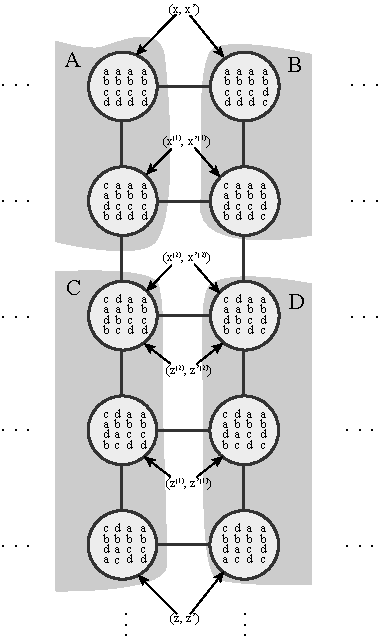
\includegraphics[width=5in]{../figures/diagram7.pdf}
	%         \caption{A visual example of a manipulation path.}
	%         \label{fig:manipulation-path}
	%     \end{center}
	% \end{figure}


	We will now go through the example table step by step for the $x$ side (left half); the $z$ side is simply a mirror image of what happens in the $x$ side. At step 0 we have $x^{(0)} = x$ because we specified above that our initial value was $(x^{(0)}, x^{\prime(0)}) = (x,x')$. At step 1 we first use Equation to essentially copy over every index from step 0 except index 1 (because it is the $k$\textsuperscript{th} index during this step). We then apply Equation to index 1 to get $y_1$. At step 2 we again use Equation to copy over every index from step 1 except for index 2 for which we use Equation to get $y_2$. We don't modify the last two indices because these are the only ones on which $x, x'$ and $z, z'$ differ: recall that $(x, x') \in B_{n-1}^{a,b}$ and $(z, z') \in B_{n}^{c,d}$.

	\begin{lemma}[Lemma 5.1 of Isaksson, Kindler, and Mossel]
		For any SCF $f$, distinct $i, j \in \{1, \ldots, n\}$ and distinct alternatives $a, b, c, d \in C$ there exists a mapping $h : B_i^{a,b}(f) \times B_j^{c,d}(f) \rightarrow M$ where
		\[
			M = \{x \in P \mid f \text{ is manipulable at x}\}
		\]
		such that for any $x \in M$
		\[
			|h^{-1}(x)| \le 2n(m!)^{n+4}
		\]
	\end{lemma}
	\begin{proof}
		Without loss of generality, let $i = n - 1$ and $j = n$. We construct a manipulation path between $(x, x') \in B_i^{a,b}(f)$ and $(z, z') \in B_j^{c,d}(f)$. Notice that $(x, x')$ takes the values $(a, b)$ while $(z, z')$ takes the values $(c, d)$ because $f(x) = a$, $f(x') = b$, $f(z) = c$, and $f(z') = d$. Our claim is that along this manipulation path is an edge $(u, u'), (v, v')$ such that either
		\begin{enumerate}
			\item at least one of $u, u', v, v'$ is a manipulation point
			\item $f$ takes on at least three values on the points $u, u', v, v'$.
		\end{enumerate}
		In explanation, notice that there are at most three possible situations, and at least one of the above claims holds for each:
		\begin{itemize}
			\item On the first half of the path the value of the pair changes from $(a, b)$ to something else. If the first value changes to $b$ or the second value changes to $a$ then we have a manipulation point because the ranking of $a, b$ doesn't change on the first half of the path. Otherwise the values change to something other than $a$ or $b$, so $f$ takes at least three values at this point.
			\item On the second half of the path the value of the pair changes from $(c, d)$ to something else --- moving from the end towards the middle. If the first value changes to $d$ or the second value changes to $c$ then we have a manipulation point because the ranking of $c, d$ doesn't change on the second half of the path. Otherwise the values change to something other than $c$ or $d$, so $f$ takes at least three values at this point.
			\item The middle edge $(x^{(n-2)}, x^{\prime(n-2)}), (z^{(n-2)}, z^{\prime(n-2)})$ connects a pair with values $(a, b)$ and $(c, d)$. Clearly $f$ takes on at least three values at this point.
		\end{itemize}

		Notice that $u, u', v, v'$ agree in all but two indices which will be either $\{n - 1, k\}$, $\{n, k\}$, or $\{n - 1, n\}$ depending on whether $(u, u'), (v, v')$ is on the first half, on the second half, or is the middle edge of the path respectively. For example, if $(u, u'), (v, v')$ is on the first half of the path $u, u'$ and $v, v'$ will both differ on the $n - 1$ index because both pairs are in $B^{a,b}_{n-1}$. Additionaly, $u, v$ and $u', v'$ will each differ on $k$\textsuperscript{th} index because of the definition of the manipulation path.

		We claim that there exists a manipulation point $h((x, x'), (z, z')) = y$ which only differs from $u, u', v, v'$ on two indices. If Case 1 above holds, then we can let $y$ be whichever one of $u, u', v, v'$ is a manipulation point.

		If Case 2 holds then we apply the Gibbard-Satterthwaite to a restricted version of $f$, which we will call $f'$, which is $f$ restricted to the two indices on which $u, u', v, v'$ differ. We call these indices $k, p$. First we define a mapping $g : L(C)^2 \rightarrow L(C)^n$ which maps profiles from $f'$ to $f$.
		\begin{align*}
			g(x)_q &= u_q \,\,\, \forall q \notin \{k, p\} \\
			g(x)_k &= x_1 \\
			g(x)_p &= x_2.
		\end{align*}
		We define the set of alternatives to be $C$ where $|C| = m$ and we define $f' : L(C)^2 \rightarrow C$ such that
		\[
			f'(x) = f(g(x)).
		\]
		If we apply the Gibbard-Satterthwaite theorem \cite{gibbard1973manipulation, satterthwaite1975strategy} to $f'$ we will see that $f'$ is manipulable since it is not a dictator and it takes on at least 3 values (because Case 2 holds). Therefore some $x$ is a manipulation point for $f'$, so $g(x)$ is a manipulation point of $f$. And in fact $g(x)$ differs from $u, u', v, v'$ on only two indices so $y = g(x)$.

		The final step in the proof is to count the maximum number of pairs that could have lead to the manipulation point $y$ and that will be simply the number of inverses of the mapping function: $|h^{-1}(f)|$. To begin with, we know that the length of the manipulation path between $(x, x')$ and $(z, z')$ is $2n - 3$. This gives us $2n - 3$ possibilities for $(u, u'), (v, v')$. In addition, given $y$ there are at most $(q!)^2$ possibilities for $u$ because it differs from $y$ on at most two indices. We find that there are at most $(q!)^n$ possibilities for $x$ and $z$ as follows. For any $k \in \{1, \ldots, n\}$ we will have either:
		\begin{itemize}
			\item $u_k = x_k$ if $u$ is on the first half of the path and $k$ is an index that hasn't been updated --- by update we mean that it has been made to conform to $x_k =_{\{a,b\}} u_k =_{\overline{\{a,b\}}} z_k$. In this case there are $q!$ possibilities for $z_k$ because it can be any preference list.
			\item $u_k = z_k$ if $u$ is on the second half of the path and $k$ is an index that hasn't been updated. In this case there are $q!$ possibilities for $x_k$ because it can be any preference list.
			\item $x_k =_{\{a,b\}} u_k =_{\overline{\{a,b\}}} z_k$ if $k$ is an index that has been updated. In this case there are $\frac{q!}{2}$ possibilities for $x_k$ because only the order of $a, b$ needs to match $u_k$, and there are $2$ possibilities for $z_k$ because the order of every alternative besides $a, b$ needs to match $u_k$.
		\end{itemize}
		No matter which of the previous cases hold for each $k$, the total number of possibilities for $x$ and $z$ is still bounded above by $(q!)^n$.

		Lastly, given $x$ and $z$ there are at most $q!$ possibilitites for each of $x'$ and $z'$ respectively, since edges of the border set differ only in one index. Summing these we get:
		\begin{align*}
			|h^{-1}| &\le (2n - 3)(q!)^2(q!)^n(q!)(q!) \\
			|h^{-1}| &\le (2n - 3)(q!)^{n+4}.
		\end{align*}

	\end{proof}

	In 2011 Friedgut et al. removed the neutrality constraint from their original theorem, and added an author \cite{friedgut2011quantitative}.

	Mossel and R\'{a}cz \cite{mossel2011quantitative} took ideas from these two proofs and created a unified proof with the same results as Isaksson, Kindler, and Mossel, but without the neutrality constraint. This is a very useful result.

























We study manipulation in election systems, looking specifically at random manipulation, and basing our work on the results of Friedgut, Kalai, and Nisan \cite{friedgut2008elections} and Xia and Conitzer \cite{xia2008sufficient}. Note that we cite the original work by Friedgut et al. \cite{friedgut2008elections} to compare it to the work by Xia and Conitzer \cite{xia2008sufficient}. However, a journal version has recently been published which loosens some of the original constraints \cite{friedgut2011quantitative} which we will describe in the Topic Area section. We will analyze these results and attempt to improve upon them by generalizing the results of Friedgut, Kalai, and Nisan, or loosening the conditions of Xia and Conitzer.  These authors condition their results on voting rules having certain properties, and we intend to look at what happens when these conditions are replaced by stronger or weaker conditions. We would also like to tighten the bounds given by these two papers by a constant factor or by making them depend of the number of candidates.

Though election systems have traditionally been used in politics, they have also been applied to many other situations. Election systems are used in schools to elect board members, and they are used in businesses for stock holders to vote on the direction of a company. Recently, artificial intelligence systems have been holding elections when a group of intelligent agents need to reach a common consensus \cite{ephrati1991clarke, ephrati1993multi, pennock2000social, dwork2001rank, fagin2003efficient}, and in internet page ranking algorithms for search engines \cite{chevaleyre2007short}.

Because election systems are so widespread and are crucial for the functioning of society, it is beneficial to study their nature along with their strengths and weaknesses. Election systems have been studied academically since as early as the 13th century \cite{hägele2001llull}, but more recently they have been scrutinized by the computer science community in the fields of theory and artificial intelligence.


\section{Overview of Hypotheses}

We will attempt to generalize the work of Friedgut et al. \cite{friedgut2008elections} and Xia and Conitzer \cite{xia2008sufficient}. This will include attempting to extend the results of Friedgut et al. \cite{friedgut2008elections} to include elections with more than three candidates. We will also extend the results of Xia and Conitzer \cite{xia2008sufficient} to capture more common voting systems by relaxing their conditions and still proving the same results. We believe that the worst case bound for random manipulation can be tightened by a constant or by depending on the number of candidates.
